\documentclass[conference]{IEEEtran}
\IEEEoverridecommandlockouts
\usepackage[T1]{fontenc}
\usepackage{booktabs}
\usepackage{graphicx}
\usepackage{amsmath,amssymb}
\usepackage{array}
\usepackage{url}
\usepackage[hidelinks]{hyperref}
\usepackage{enumitem}
\usepackage{microtype}
\setlist[itemize]{leftmargin=*,nosep}
\begin{document}

\title{Predicting Late Sprint Closure and Unfinished Committed Scope from Reconstructed Jira Histories}

\author{\IEEEauthorblockN{Hani AbuSharkh}
\IEEEauthorblockA{Higher Colleges of Technology\\United Arab Emirates\\habusharkh@hct.ac.ae}
\and
\IEEEauthorblockN{Maryam Hanif}
\IEEEauthorblockA{United Arab Emirates University\\United Arab Emirates\\700052696@uaeu.ac.ae}
\and
\IEEEauthorblockN{Rafat Damseh}
\IEEEauthorblockA{United Arab Emirates University\\United Arab Emirates\\rdamseh@uaeu.ac.ae}}
\maketitle

\begin{abstract}
Repository data are useful at Sprint Planning only if the features reflect what was known at that time. We examine two repository-derived outcomes in eight TAWOS projects: late sprint closure and unfinished scope that was committed when the sprint began. Sprint membership and story points are reconstructed from Jira change history, with a documented static fallback when no relevant history is recorded. After removing nonclosed and invalid sprint rows and one genuine cold start per project, 2,602 sprints remain. Late closure is only moderately discriminable: random forest reaches 0.705 ROC-AUC on the main time-ordered split, with a project-cluster 95\% interval of 0.604--0.783. For nonempty sprints, a simple scope-only logistic model reaches 0.885 ROC-AUC, compared with 0.852 for random forest. The simpler model therefore captures most of the useful spillover ranking signal. Provenance matters: when the analysis is restricted to the much smaller subset in which every committed item has observed Sprint and Story Points history, the random-forest AUC falls to 0.652 on 110 test sprints. Results are also reported across multiple temporal cut points and held-out projects. The evidence supports cautious retrospective ranking of these two outcomes, not a deployment-ready Scrum decision system.
\end{abstract}

\begin{IEEEkeywords}
Scrum, sprint analytics, Jira, temporal provenance, software analytics, machine learning, data leakage
\end{IEEEkeywords}

\section{Introduction}
Sprint Planning is one of the few points in Scrum where the team can still change the amount and shape of the work before execution begins. Most operational warning signs arrive later: blockers accumulate, the burndown stalls, or unfinished work becomes obvious during the Daily Scrum. That timing makes an early repository-based signal attractive, but it also creates a strict data requirement. A model evaluated at sprint start must use the state of the repository at sprint start, not the final state stored after weeks or months of edits.

We focus on two narrow outcomes. The first is \emph{late sprint closure}: Jira records the sprint as completed more than one day after its planned end. The second is \emph{unfinished committed scope}: at least one issue that belonged to the sprint at its start is unresolved by the planned end. Neither outcome is a general measure of Scrum success or team quality. They are observable repository events that can be studied consistently across projects.

A final Jira export is not a historical snapshot. Issues move between sprints, estimates change, and some records are created after a sprint has already started. To reduce that timing error, we reconstruct Sprint membership and Story Points from timestamped TAWOS change records. When a field has no relevant history, the static value is used as a fallback and is reported as such. We exclude developer count because assignee-at-start cannot be reconstructed reliably from the available export.

Four questions guide the analysis: (1) how much ranking signal is present for late closure and unfinished committed scope; (2) whether a simple scope model performs as well as more flexible models; (3) how stable the findings are across projects and temporal cut points; and (4) how sensitive the results are to incomplete historical provenance and common leakage mistakes.

\section{Related Work}
Machine learning in Agile software analytics has most often been used for effort estimation, sprint monitoring, and project-risk support. Choetkiertikul et al.~\cite{choetkiertikul2019} estimated story points from Jira text, while Shankar et al.~\cite{shankar2026} compared several predictive models for Agile effort data. P\'erez Castillo et al.~\cite{perezcastillo2024} used burndown-derived features to classify sprint performance; those features are informative during the sprint but are not available at its start. Obike et al.~\cite{obike2025} studied sprint deliverability with an ensemble approach, and Almalki~\cite{almalki2025} examined interpretable AI support for Agile project risk.

Our emphasis is different. The main concern is the timestamp attached to each predictor. We reconstruct selected fields at the prediction time, retain transparent baselines alongside random forest and XGBoost, and report both within-project temporal performance and transfer to a held-out project. The aim is to estimate what can reasonably be learned from repository history without treating final-state data as if they had been known in advance.

The closest studies also differ in what they predict and when their features become available. Table~\ref{tab:related} summarizes the comparison that motivated the design choices here.

\begin{table}[t]
\centering\scriptsize
\caption{Selected related work and the evaluation gap}
\label{tab:related}
\setlength{\tabcolsep}{2.2pt}
\begin{tabular}{@{}p{1.55cm}p{1.55cm}p{1.05cm}p{1.1cm}@{}}
\toprule
Study & Main task & Sprint-start features & Project holdout\\
\midrule
Choetkiertikul et al. & Story-point estimation & Yes & No\\
Shankar et al. & Effort/time estimation & Yes & No\\
P\'erez Castillo et al. & Sprint performance & No; burndown & No\\
Obike et al. & Deliverability & Intended & No\\
Almalki & Agile risk support & Historical & No\\
This work & Closure / unfinished scope & Reconstructed & Yes\\
\bottomrule
\end{tabular}
\end{table}

\section{Data and Reconstruction}
TAWOS~\cite{tawosi2022} contains public Jira data from open-source Agile projects. Eight projects with at least 30 sprint records are retained. The raw subset has 2,657 sprint rows and 145,309 issues. Table~\ref{tab:flow} shows the cleaning path. FUTURE and ACTIVE rows are removed before labels are built because their closure outcome is not observed. Three CLOSED rows with impossible timestamps are also removed. Historical features require a predecessor, so the first eligible sprint in each project is the only cold start excluded. The model frame contains 2,602 sprints.

\begin{table}[t]
\centering\scriptsize
\caption{Sprint flow by project}
\label{tab:flow}
\setlength{\tabcolsep}{2.1pt}
\begin{tabular}{@{}p{2.0cm}rrrrr@{}}
\toprule
Project & Raw & Nonclosed & Invalid & Modeled & Nonempty\\
\midrule
Apache Mesos & 227 & 2 & 0 & 224 & 133\\
Appcelerator Studio & 163 & 0 & 0 & 162 & 129\\
Confluence Cloud & 477 & 10 & 2 & 464 & 197\\
Confluence Server & 565 & 7 & 0 & 557 & 289\\
Lsstcorp Data & 396 & 8 & 0 & 387 & 309\\
Mule & 311 & 13 & 0 & 297 & 228\\
Titanium SDK & 301 & 1 & 0 & 299 & 241\\
Titanium Mobile & 217 & 3 & 1 & 212 & 165\\
\bottomrule
\end{tabular}
\end{table}

For each issue, the reconstruction uses two sprint identifier maps because TAWOS stores database sprint IDs and Jira sprint IDs in different places. The latest known state is walked backward through field changes until the target sprint-start timestamp is reached. An issue is counted as committed only if it existed by that timestamp, belonged to the sprint then, and had not already been resolved. The same procedure reconstructs story points. Across the eligible sprints, the process yields 20,603 issue-sprint commitments.

\begin{table}[t]
\centering\scriptsize
\caption{Commitment provenance by project}
\label{tab:provproj}
\setlength{\tabcolsep}{2.2pt}
\begin{tabular}{@{}p{2.0cm}rrr@{}}
\toprule
Project & Sprint hist. & Sprint fallback & SP hist.\\
\midrule
Apache Mesos & 96.4\% & 3.6\% & 56.8\%\\
Appcelerator & 95.8\% & 4.2\% & 87.2\%\\
Confluence Cloud & 54.1\% & 45.9\% & 11.2\%\\
Confluence Server & 99.1\% & 0.9\% & 54.4\%\\
Lsstcorp Data & 92.4\% & 7.6\% & 41.8\%\\
Mule & 92.3\% & 7.7\% & 77.0\%\\
Titanium SDK & 97.1\% & 2.9\% & 68.3\%\\
Titanium Mobile & 93.6\% & 6.4\% & 54.0\%\\
\bottomrule
\end{tabular}
\end{table}

The fallback rule deserves explicit attention. If no Sprint change is recorded for an issue, the static sprint value is treated as unchanged; the same rule is used for Story Points. That assumption is plausible but not verifiable for every record. Coverage varies by project, so we report commitment-level provenance and repeat the spillover analysis on stricter subsets with observed history.

The reconstruction follows a deterministic sequence. Change events are sorted by issue, timestamp, and change ID. The state begins from the latest recorded value and is rolled backward to each sprint start. A change recorded exactly at the start timestamp is treated as available at the start; only later changes are undone. Multi-sprint Jira values are parsed as sets, and unknown sprint identifiers are ignored if they do not map to a retained sprint.

\begin{enumerate}[leftmargin=*,nosep]
\item Load Sprint, Issue, and Change\_Log rows for the eight projects.
\item Remove nonclosed and invalid sprint rows before any labels are created.
\item Build project-specific maps for database sprint IDs and Jira sprint IDs.
\item Reconstruct Sprint membership and Story Points at each sprint's start time.
\item Keep an issue only if it existed by the start time, belonged to that sprint, and had not already been resolved.
\item Aggregate committed issues, committed points, completed issues, delivered points, and carryover.
\item Build labels and historical features, then remove one genuine cold start per project.
\end{enumerate}

\begin{figure}[t]
\centering
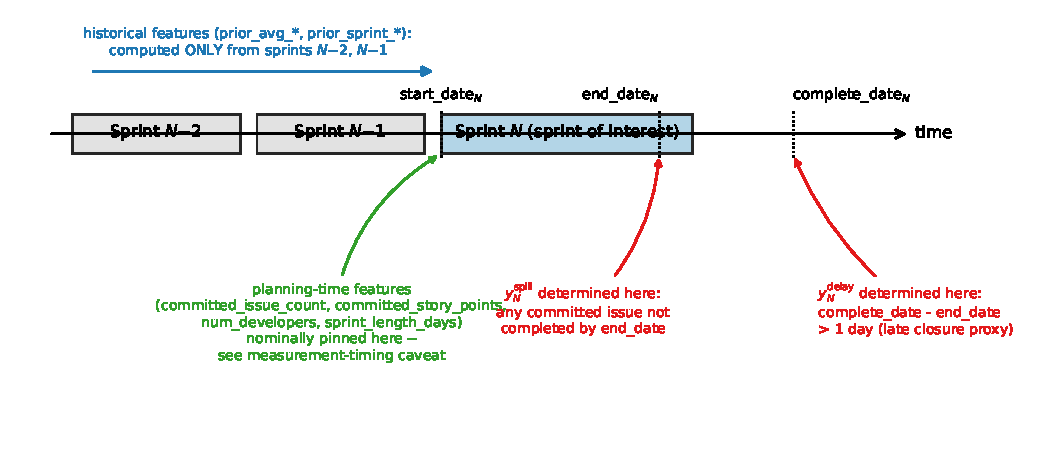
\includegraphics[width=\columnwidth]{dataflow_timing.pdf}
\caption{Data timing and reconstruction used before model fitting.}
\label{fig:dataflow}
\end{figure}

\section{Methods}
\subsection{Outcomes and features}
Late closure is defined as
\begin{equation}
y^{late}_s = \mathbb{1}[c_s-e_s>1\ \mathrm{day}],
\end{equation}
where $c_s$ is Jira's completion timestamp and $e_s$ is the planned end timestamp. Missing completion dates are never coded as on time; the corresponding nonclosed sprints are excluded before modeling.

Unfinished committed scope is defined as
\begin{equation}
y^{spill}_s = \mathbb{1}[u_s>0],
\end{equation}
where $u_s$ is the number of sprint-start committed issues unresolved by the planned end. The main conditional analysis excludes reconstructed zero-scope sprints because they are negative by construction.

Current-sprint predictors are committed issue count, committed story points, and planned sprint length. Historical predictors summarize recent delivered points, recent completion ratio, prior carryover, and the immediately preceding sprint's completion ratio. Project identity is included only in the full models. The scope-only logistic model uses current scope and sprint length, with no project identity or historical variables.

\subsection{Models, thresholds, and validation}
\begin{table}[t]
\centering\scriptsize
\caption{Predictor groups used in the final analysis}
\label{tab:features}
\setlength{\tabcolsep}{2.3pt}
\begin{tabular}{@{}p{2.2cm}p{4.55cm}@{}}
\toprule
Group & Variables\\
\midrule
Current scope & committed issue count; committed story points; planned sprint length\\
Recent history & mean delivered points over prior 3 sprints; mean completion ratio over prior 3; prior carryover; prior sprint completion ratio\\
Context & one-hot project identity in full models only\\
\bottomrule
\end{tabular}
\end{table}

We compare prevalence baselines, count-only and scope-only logistic regression, random forest, and XGBoost. Random forest uses 300 trees, maximum depth 5, and minimum leaf size 3. XGBoost uses 300 trees, maximum depth 4, learning rate 0.05, and log-loss optimization. Logistic regression and random forest use balanced class weights; XGBoost is unweighted. Precision, recall, and F1 use a fixed 0.5 threshold chosen before testing. ROC-AUC is the main ranking metric. Brier score and reliability bins are reported descriptively because class weighting changes probability calibration.

\begin{table}[t]
\centering\scriptsize
\caption{Model settings held fixed across the reported runs}
\label{tab:settings}
\setlength{\tabcolsep}{2.4pt}
\begin{tabular}{@{}p{1.65cm}p{5.1cm}@{}}
\toprule
Model & Main settings\\
\midrule
Logistic regression & standardized numeric features; balanced class weights\\
Random forest & 300 trees; max depth 5; min leaf 3; balanced class weights\\
XGBoost & 300 trees; max depth 4; learning rate .05; log-loss objective\\
\bottomrule
\end{tabular}
\end{table}

The main temporal split trains on the earlier 70\% of each project's modeled sprints and tests on the later 30\%. Additional forward splits use 50/50, 60/40, and 80/20 boundaries. Leave-one-project-out (LOPO) trains the model on seven projects and tests it on the eighth. Historical features for the held-out project still come from that project's own earlier sprints, so LOPO measures cross-project transfer with local history, not a complete new-project cold start.

Uncertainty for the main time-ordered results is estimated by resampling whole projects rather than individual sprint rows. This keeps within-project dependence visible. Feature evidence uses permutation importance on held-out data rather than relying only on tree impurity importance.

\section{Results}
\begin{table*}[t]
\centering\scriptsize
\caption{Project-level modeled cohort and outcome prevalence}
\label{tab:projectprev}
\setlength{\tabcolsep}{3.4pt}
\begin{tabular}{@{}lrrrrrr@{}}
\toprule
Project & Modeled & Zero scope & Late positives & Late rate & Nonempty & Spillover positives / rate\\
\midrule
Apache Mesos & 224 & 91 & 66 & .295 & 133 & 128 / .962\\
Appcelerator Studio & 162 & 33 & 73 & .451 & 129 & 121 / .938\\
Confluence Cloud & 464 & 267 & 186 & .401 & 197 & 187 / .949\\
Confluence Server & 557 & 268 & 171 & .307 & 289 & 255 / .882\\
Lsstcorp Data & 387 & 78 & 226 & .584 & 309 & 304 / .984\\
Mule & 297 & 69 & 57 & .192 & 228 & 200 / .877\\
Titanium SDK & 299 & 58 & 179 & .599 & 241 & 228 / .946\\
Titanium Mobile & 212 & 47 & 48 & .226 & 165 & 152 / .921\\
\bottomrule
\end{tabular}
\end{table*}

Project prevalence is highly uneven. Late closure ranges from 19.2\% in Mule to 59.9\% in Titanium SDK. Conditional spillover is common in every project and exceeds 87\% throughout. This heterogeneity matters for both evaluation and interpretation: pooled threshold metrics can hide a project that behaves very differently from the average, while a high conditional prevalence can make an always-positive classifier look deceptively strong on F1.

\subsection{Descriptive context}
The reconstructed cohorts already show why the two outcomes behave differently. Across all 2,602 modeled sprints, the mean committed issue count is 7.9 and the mean committed story-point total is 35.0. Late-closure positives have somewhat larger scope and longer planned duration, but the separation is modest. Spillover positives are much larger than spillover negatives because many negatives are reconstructed zero-scope sprints. That structural difference motivates reporting the nonempty-sprint task separately.

\begin{table}[t]
\centering\scriptsize
\caption{Planning-time feature means over 2,602 modeled sprints}
\label{tab:descriptive}
\setlength{\tabcolsep}{3.2pt}
\begin{tabular}{@{}lrrr@{}}
\toprule
Group & Issues & Story points & Days\\
\midrule
Overall & 7.9 & 35.0 & 13.8\\
Late closure = 0 & 7.3 & 32.9 & 13.2\\
Late closure = 1 & 8.8 & 38.3 & 14.6\\
Spillover = 0 & 0.3 & 1.1 & 12.8\\
Spillover = 1 & 12.9 & 57.0 & 14.4\\
\bottomrule
\end{tabular}
\end{table}

\subsection{Main comparison}
Table~\ref{tab:main} contains the main 70/30 test results. Late closure has 246 positives among 786 test sprints. Random forest reaches 0.705 ROC-AUC and 0.562 F1. The scope-only logistic model is much weaker at 0.530 AUC, which suggests that project and historical context add some ranking information for this outcome. Even so, the discrimination is moderate rather than strong.

The nonempty-spillover test set contains 482 positives among 511 sprints. An always-positive classifier therefore has F1=0.971, illustrating why F1 is a poor headline for this task. Scope-only logistic regression reaches 0.885 ROC-AUC, while the full random forest reaches 0.852. The result is parsimonious: larger initial scope carries most of the usable ranking signal, and the additional complexity of the full model does not improve AUC on the main split.

\begin{table*}[t]
\centering\scriptsize
\caption{Main time-ordered test results. Thresholded metrics use a fixed 0.5 threshold.}
\label{tab:main}
\setlength{\tabcolsep}{3.2pt}
\begin{tabular}{@{}llrrrrrrr@{}}
\toprule
Outcome & Model & n & Pos. & Prev. & F1 & ROC-AUC & PR-AUC & Brier\\
\midrule
Late closure & Always positive & 786 & 246 & .313 & .477 & .500 & .313 & .687\\
Late closure & Scope-only LR & 786 & 246 & .313 & .336 & .530 & .373 & .244\\
Late closure & Random forest & 786 & 246 & .313 & .562 & .705 & .458 & .223\\
Late closure & XGBoost & 786 & 246 & .313 & .535 & .695 & .478 & .206\\
\midrule
Spillover, nonempty & Always positive & 511 & 482 & .943 & .971 & .500 & .943 & .057\\
Spillover, nonempty & Count-only LR & 511 & 482 & .943 & .650 & .881 & .989 & .234\\
Spillover, nonempty & Scope-only LR & 511 & 482 & .943 & .696 & .885 & .992 & .230\\
Spillover, nonempty & Random forest & 511 & 482 & .943 & .875 & .852 & .990 & .136\\
\bottomrule
\end{tabular}
\end{table*}

\begin{table}[t]
\centering\scriptsize
\caption{Project-cluster 95\% intervals on the main split}
\label{tab:cluster}
\setlength{\tabcolsep}{2.4pt}
\begin{tabular}{@{}llcc@{}}
\toprule
Outcome & Model & F1 interval & AUC interval\\
\midrule
Late closure & RF & [.317,.688] & [.604,.783]\\
Spillover & Scope LR & [.482,.823] & [.820,.922]\\
Spillover & RF & [.804,.923] & [.797,.914]\\
\bottomrule
\end{tabular}
\end{table}

\subsection{Uncertainty and temporal stability}
Project-cluster resampling gives a 95\% AUC interval of 0.604--0.783 for late-closure random forest. For conditional spillover, the interval is 0.820--0.922 for scope-only logistic regression and 0.797--0.914 for random forest. The overlap reinforces the main point: the scope-only model is competitive, and small ranking differences should not be treated as precise model superiority.

Forward temporal splits tell a similar story. Late-closure random-forest AUC ranges from 0.669 at the 50/50 boundary to 0.711 at 80/20. Conditional-spillover random-forest AUC remains between 0.846 and 0.856. Scope-only logistic regression ranges from 0.865 to 0.887 over the same conditional splits. The broad conclusion is not tied to one 70/30 cutoff.

\begin{table}[t]
\centering\scriptsize
\caption{Temporal sensitivity. AUC values on forward test periods.}
\label{tab:temporal}
\setlength{\tabcolsep}{3pt}
\begin{tabular}{@{}lrrrr@{}}
\toprule
Outcome/model & 50/50 & 60/40 & 70/30 & 80/20\\
\midrule
Late closure, RF & .669 & .685 & .705 & .711\\
Spillover, scope LR & .865 & .887 & .885 & .878\\
Spillover, RF & .846 & .856 & .852 & .853\\
\bottomrule
\end{tabular}
\end{table}

\subsection{Cross-project transfer and feature evidence}
LOPO results vary substantially by project. Late-closure random-forest AUC ranges from 0.531 to 0.780. Conditional-spillover random forest ranges from 0.706 to 0.950. Table~\ref{tab:lopo} includes denominators because project prevalence differs considerably. A model that transfers well to one project may be only modestly useful on another.

\begin{table}[t]
\centering\scriptsize
\caption{LOPO random-forest AUC with test denominators}
\label{tab:lopo}
\setlength{\tabcolsep}{2.0pt}
\begin{tabular}{@{}p{1.95cm}rrrr@{}}
\toprule
Project & Late n/pos & AUC & Spill n/pos & AUC\\
\midrule
Apache Mesos & 224/66 & .572 & 133/128 & .858\\
Appcelerator & 162/73 & .780 & 129/121 & .950\\
Confluence Cloud & 464/186 & .745 & 197/187 & .706\\
Confluence Server & 557/171 & .604 & 289/255 & .768\\
Lsstcorp Data & 387/226 & .557 & 309/304 & .937\\
Mule & 297/57 & .561 & 228/200 & .809\\
Titanium SDK & 299/179 & .574 & 241/228 & .873\\
Titanium Mobile & 212/48 & .531 & 165/152 & .780\\
\bottomrule
\end{tabular}
\end{table}

\begin{figure}[t]
\centering
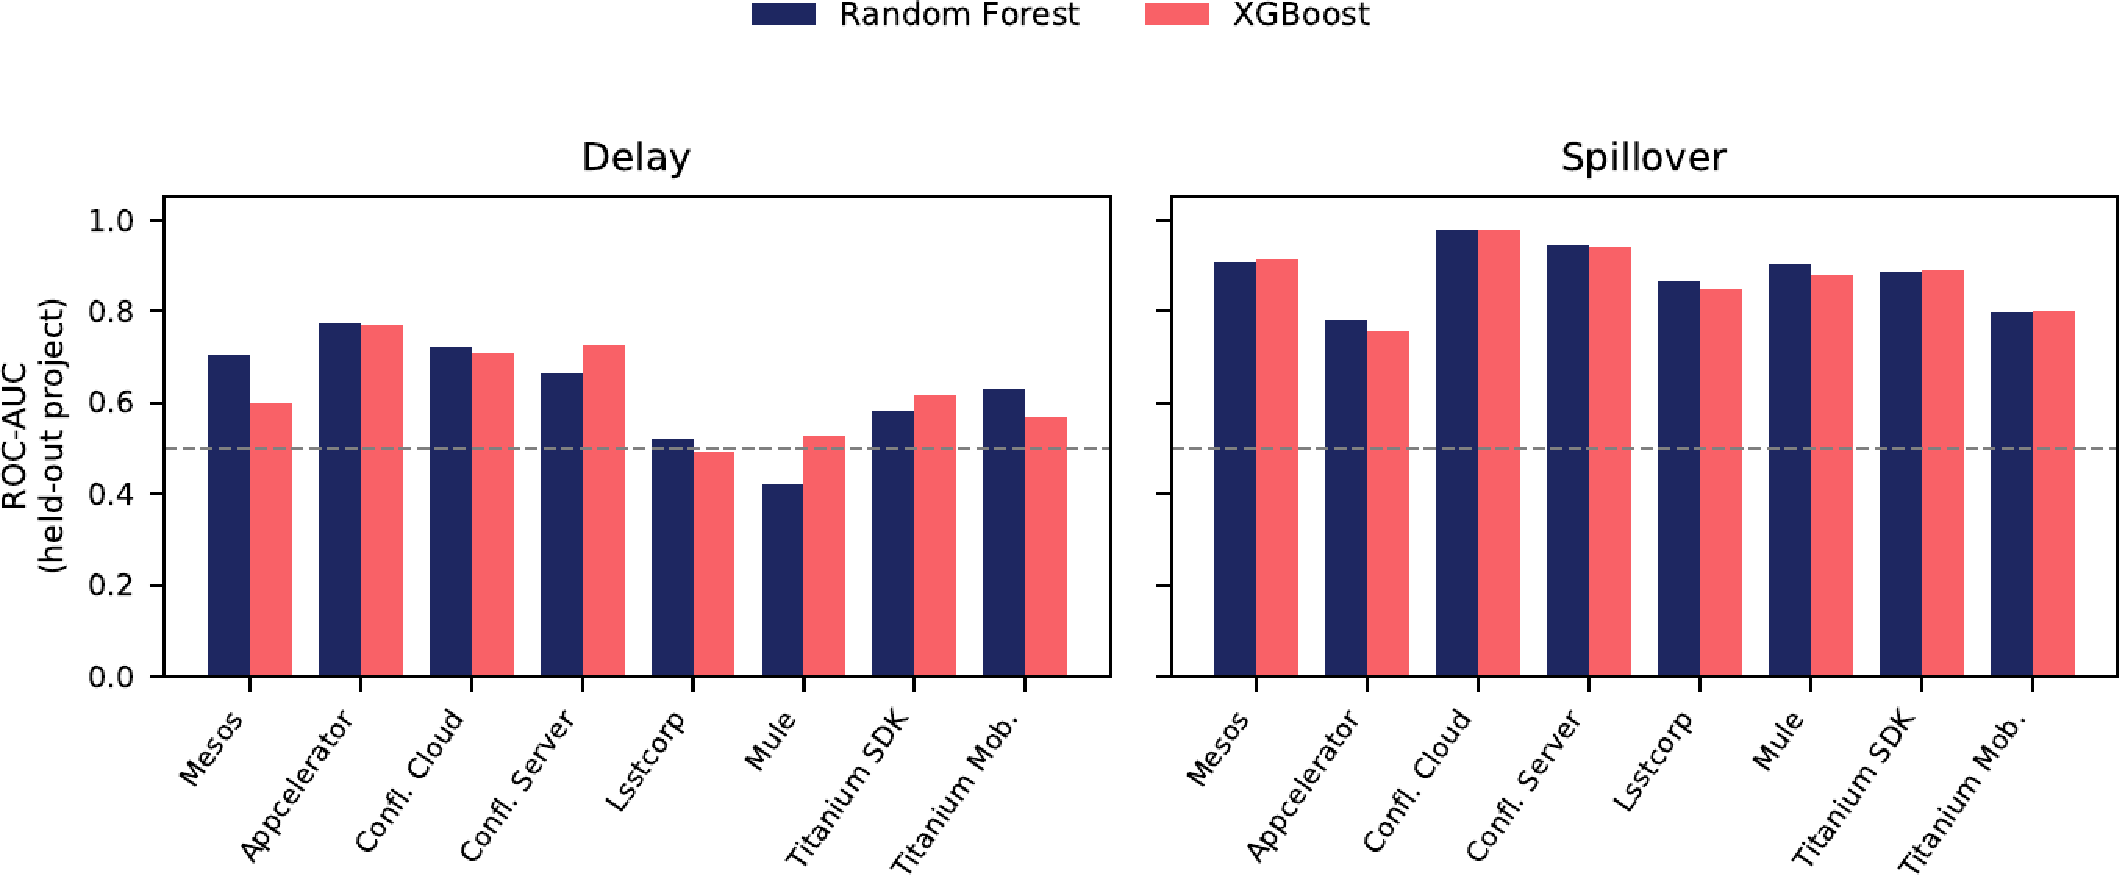
\includegraphics[width=\columnwidth]{lopo_auc_by_project.pdf}
\caption{Held-out-project AUC by project.}
\label{fig:lopo}
\end{figure}

Held-out permutation importance clarifies what the random forest uses. Project identity (mean AUC drop 0.104) and sprint length (0.077) matter most for late closure. For conditional spillover, committed issue count dominates with a mean AUC drop of 0.220; the next largest positive drop is only 0.021. This pattern agrees with the scope-only baseline and makes the result easier to interpret.

A feature-group ablation gives the same qualitative picture. For late closure, random forest changes little when only planning-time variables are kept (AUC 0.706 versus 0.705 for the full model), and removing explicit project identity still gives 0.696. For full-population spillover, planning-only random forest is essentially unchanged at 0.987 AUC, whereas history-only performance falls to 0.697. Historical features therefore do not rescue the spillover task once initial scope is known.

\begin{table}[t]
\centering\scriptsize
\caption{Random-forest feature-group ablation, F1 (AUC)}
\label{tab:abshort}
\setlength{\tabcolsep}{3.0pt}
\begin{tabular}{@{}lll@{}}
\toprule
Configuration & Late closure & Full spillover\\
\midrule
Full & .562 (.705) & .969 (.986)\\
Planning only & .588 (.706) & .969 (.987)\\
History only & .377 (.625) & .680 (.697)\\
No project identity & .542 (.696) & .969 (.989)\\
\bottomrule
\end{tabular}
\end{table}

\subsection{Provenance sensitivity}
The main reconstruction combines observed change history with static fallback when no change is recorded. Coverage is uneven. For example, 96.4\% of Apache Mesos commitments have observed Sprint history, compared with 54.1\% for Confluence Cloud. Story-point history is sparser still.

Table~\ref{tab:prov} restricts the conditional spillover analysis to higher-provenance subsets. Requiring observed Sprint history for every committed item leaves 1,174 modeled sprints and 356 test sprints; scope-only logistic regression remains at 0.875 AUC and random forest at 0.850. Requiring both Sprint and Story Points history leaves only 358 modeled sprints and 110 test sprints. On this stricter subset, scope-only AUC is 0.772 and random-forest AUC is 0.652. The smaller sample makes the estimate less stable, but the drop is important: provenance quality affects the measured difficulty of the task.

\begin{table}[t]
\centering\scriptsize
\caption{Conditional-spillover sensitivity to observed history}
\label{tab:prov}
\setlength{\tabcolsep}{2.4pt}
\begin{tabular}{@{}llrrrr@{}}
\toprule
Subset & Model & Test n & Pos. & F1 & AUC\\
\midrule
Observed Sprint & Scope LR & 356 & 335 & .719 & .875\\
Observed Sprint & RF & 356 & 335 & .875 & .850\\
Sprint + SP history & Scope LR & 110 & 94 & .652 & .772\\
Sprint + SP history & RF & 110 & 94 & .876 & .652\\
\bottomrule
\end{tabular}
\end{table}

\subsection{Calibration and leakage checks}
\begin{figure}[t]
\centering
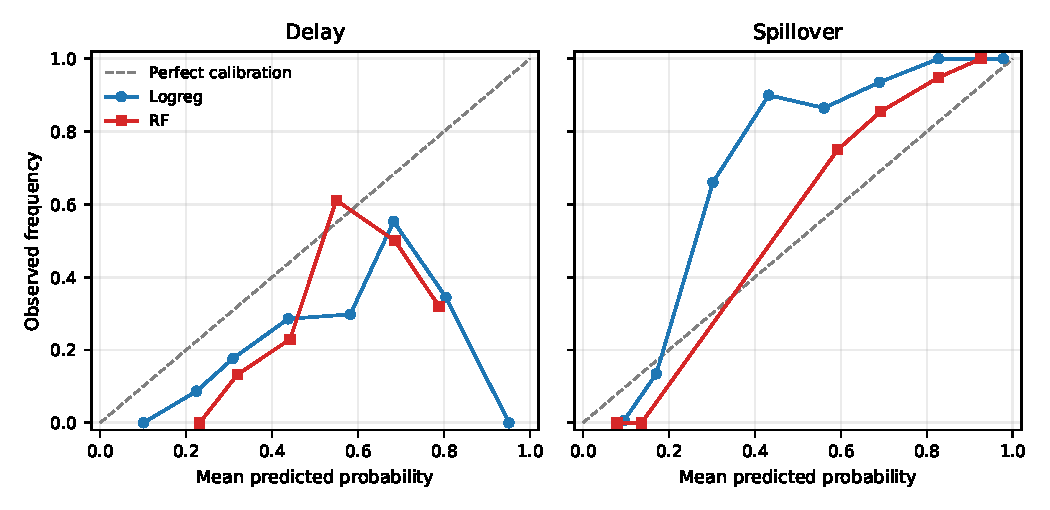
\includegraphics[width=\columnwidth]{calibration_reliability.pdf}
\caption{Reliability bins for selected random-forest scores.}
\label{fig:cal}
\end{figure}

\begin{table}[t]
\centering\scriptsize
\caption{Selected random-forest reliability bins}
\label{tab:calbins}
\setlength{\tabcolsep}{2.5pt}
\begin{tabular}{@{}llrrr@{}}
\toprule
Outcome & Score bin & n & Mean & Observed\\
\midrule
Late & .3--.4 & 159 & .356 & .182\\
Late & .5--.6 & 144 & .544 & .625\\
Late & .7--.8 & 46 & .749 & .348\\
Spillover & .3--.4 & 49 & .350 & .898\\
Spillover & .7--.8 & 81 & .752 & .975\\
Spillover & .9--1.0 & 109 & .947 & 1.000\\
\bottomrule
\end{tabular}
\end{table}

\begin{table}[t]
\centering\scriptsize
\caption{Leakage demonstrations, F1 before and after the mistake}
\label{tab:leak}
\setlength{\tabcolsep}{2.6pt}
\begin{tabular}{@{}lllrr@{}}
\toprule
Outcome & Mechanism & Correct & Leaky & Change\\
\midrule
Late & Post-outcome feature & .463 & .473 & +.010\\
Late & Oversample before split & .457 & .646 & +.189\\
Spillover & Post-outcome feature & .756 & .991 & +.235\\
Spillover & Oversample before split & .972 & .972 & .000\\
\bottomrule
\end{tabular}
\end{table}

Reliability bins show that the raw model probabilities should not be read as literal risk percentages. The high prevalence of conditional spillover and the use of class weighting both contribute to that limitation. Probability scores are treated mainly as ranking outputs.

Two controlled leakage checks illustrate how evaluation choices can distort results. Adding the current sprint's own completion ratio barely changes late-closure F1 but drives spillover F1 close to one. Oversampling before the train/test split raises late-closure F1 substantially while having almost no effect on the already high-prevalence spillover task. Leakage does not create a fixed amount of inflation; the effect depends on the target and the mechanism.

\subsection{Outcome-definition sensitivity}
The broad findings are not tied to one exact threshold. For late closure, random-forest AUC is 0.696 with no grace day, 0.705 with the one-day definition, 0.685 with a three-day tolerance, and 0.626 with seven days. In the full spillover population, requiring at least two or three unfinished issues still produces AUCs of 0.984 and 0.980. A story-point completion-ratio label below 0.8 gives 0.977 AUC. These checks do not remove the provenance and prevalence concerns, but they show that the full-population separation is not created by a single arbitrary cutoff.

\begin{table}[t]
\centering\scriptsize
\caption{Selected label-sensitivity results, random forest}
\label{tab:labelsens}
\setlength{\tabcolsep}{3pt}
\begin{tabular}{@{}lrrr@{}}
\toprule
Variant & Test prevalence & F1 & AUC\\
\midrule
Late $>$0 days & .609 & .649 & .696\\
Late $>$1 day & .313 & .562 & .705\\
Late $>$3 days & .182 & .353 & .685\\
Late $>$7 days & .111 & .216 & .626\\
Spillover $\geq$2 issues & .467 & .955 & .984\\
SP completion $<$.8 & .467 & .957 & .977\\
\bottomrule
\end{tabular}
\end{table}

\subsection{Reconstruction audit}
The exported change log contains 88,364 relevant Sprint and Story Points events. At issue level, history coverage varies substantially: 38.1\% of Titanium Mobile issues have Sprint history, compared with 2.9\% in Confluence Cloud. Commitment-level coverage is higher because committed items are not a random sample of all project issues. Both project coverage and stricter subset results are reported because missing history is not uniform across the data.

Several edge cases are handled explicitly. Multi-valued Sprint fields are treated as sets. An issue can carry a historical sprint identifier that belongs to a sprint outside the retained subset; that identifier is ignored instead of being forced into a selected sprint. Missing story points contribute zero points but do not remove an otherwise valid commitment. Issues resolved before the sprint starts are excluded from planning scope because they cannot represent unresolved work at that time.

\section{Discussion}
The clearest finding is not that a complex model wins. It is that the two repository outcomes behave differently. Late closure contains a modest signal that depends on project context and sprint length, and that signal transfers unevenly. Unfinished committed scope is easier to rank, but most of that ranking comes from the amount of work present at sprint start. A transparent scope-only model is therefore a serious baseline, not a token comparison.

This distinction also narrows the practical claim. The analysis can rank historical sprints under the stated reconstruction assumptions. It does not show that a Scrum Master should act on a score, that the score improves delivery, or that the same model will calibrate well in a new organization. A sensible next step would be a prospective silent deployment in which scores are generated without changing team behavior, followed by local calibration and only then an intervention study.

The provenance sensitivity is equally important. Reconstructing timestamped fields is more defensible than using a static export, but incomplete change history remains an identification problem. The strict observed-history subset is smaller and produces weaker random-forest discrimination. Any use of the main estimate should therefore keep the fallback assumption visible.

\section{Threats to Validity}
\textit{Construct validity.} Jira's completion timestamp records sprint closure, not necessarily the moment all work finished. The spillover label is also narrow: it asks whether at least one sprint-start committed issue remains unresolved by the planned end. Neither label should be generalized to overall team performance.

\textit{Reconstruction validity.} Missing Sprint or Story Points history is handled with static fallback. The provenance tables and sensitivity analysis show how much the result depends on that choice, but they cannot recover events that were never recorded. Jira use also differs by project.

\textit{Evaluation validity.} Only eight projects are available, so project-level uncertainty is necessarily wide. LOPO retains local historical features from the held-out project and should be interpreted as transfer of the learned rule rather than a complete cold start. Thresholded metrics are affected by prevalence, especially for conditional spillover.

\textit{External validity.} The projects are open-source Jira projects. Enterprise teams may differ in staffing, backlog practice, and administrative use of sprints. Absolute performance should not be transported without local validation.

\section{Reproducibility and Audit Trail}
The artifact keeps the data preparation and modeling stages separate so that a reader can inspect the reconstruction before looking at model scores. The raw project subset consists of three CSV exports: Sprint, Issue, and the relevant Sprint/Story Points rows from Change\_Log. The reconstruction code writes the planning-time aggregates used by the models, while the analysis scripts save their outputs as CSV or JSON rather than only printing them to the console.

The main result tables can be regenerated with three commands. \texttt{python -m scripts.run\_baseline} rebuilds the principal temporal and held-out-project results. \texttt{python -m scripts.audit\_commitment\_provenance} creates the provenance summaries and the stricter-history sensitivity sets. \texttt{python -m scripts.run\_validation\_sensitivity\_analyses} produces the transparent baselines, project-cluster intervals, forward cut points, project-flow counts, held-out permutation importance, calibration bins, and the recorded software environment. Label sensitivity and leakage demonstrations are kept in separate scripts so that they do not alter the primary results.

\begin{table}[t]
\centering\scriptsize
\caption{Recorded software environment}
\label{tab:env}
\setlength{\tabcolsep}{4pt}
\begin{tabular}{@{}lr@{}}
\toprule
Component & Version\\
\midrule
Python & 3.13.5\\
NumPy & 2.3.5\\
pandas & 2.2.3\\
scikit-learn & 1.8.0\\
XGBoost & 3.1.3\\
\bottomrule
\end{tabular}
\end{table}

Automated tests cover label construction, cold-start handling, reconstruction of planning snapshots, feature creation, scope decomposition, and known leakage cases. The package also includes a manuscript-number crosswalk that points each headline statistic to the result file from which it was taken. This is a practical safeguard against one manuscript being updated while another retains an older number.

Exact bitwise agreement can still depend on operating-system and library details for tree-based learners. The reproducibility target is therefore the data-cleaning rules, reconstructed cohort, split definitions, feature construction, and reported metrics within ordinary numerical tolerance. The recorded environment in Table~\ref{tab:env} is provided to make that target as concrete as possible.

\section{Conclusion}
Reconstructed Jira history contains measurable signal for two sprint-start outcomes, but the signal is narrower than a generic ``sprint risk'' claim. Late closure is only moderately discriminable and varies across projects. For nonempty sprints, initial scope is strongly associated with unfinished work; a simple scope-only logistic model reaches 0.885 AUC and does not lose to the more complex random forest on the main split. Stricter provenance requirements reduce the sample and weaken some estimates, which makes data history part of the result rather than a footnote. The practical value of these rankings remains a question for prospective validation with real teams.


\begin{thebibliography}{9}
\bibitem{tawosi2022} V. Tawosi, A. Al-Subaihin, R. Moussa, and F. Sarro, ``A versatile dataset of agile open source software projects,'' in \emph{Proc. 19th Int. Conf. Mining Software Repositories}, 2022, pp. 707--711.
\bibitem{choetkiertikul2019} M. Choetkiertikul, H. K. Dam, T. Tran, T. T. M. Pham, A. Ghose, and T. Menzies, ``A deep learning model for estimating story points,'' \emph{IEEE Trans. Softw. Eng.}, vol. 45, no. 7, pp. 637--656, 2019.
\bibitem{shankar2026} S. P. Shankar, S. S. Chaudhari, V. Mishra, and T. Stephan, ``Intelligent techniques for predictive analytics in Agile software development,'' \emph{Scientific Reports}, vol. 16, 2026.
\bibitem{perezcastillo2024} Y. J. P\'erez Castillo, S. D. Orantes Jim\'enez, and P. O. Letelier Torres, ``Sprint management in Agile approach: Progress and velocity evaluation applying machine learning,'' \emph{Information}, vol. 15, no. 11, 2024.
\bibitem{obike2025} P. G. Obike, V. E. Ekong, and O. U. Obot, ``A novel scoring-based Agile sprint deliverability prediction and prioritization using machine learning,'' \emph{Int. J. Comput. Appl.}, vol. 187, no. 49, 2025.
\bibitem{almalki2025} S. S. Almalki, ``AI-driven decision support systems in Agile software project management,'' \emph{Systems}, vol. 13, no. 3, 2025.
\bibitem{xgboost2016} T. Chen and C. Guestrin, ``XGBoost: A scalable tree boosting system,'' in \emph{Proc. ACM SIGKDD}, 2016, pp. 785--794.
\bibitem{rf2001} L. Breiman, ``Random forests,'' \emph{Mach. Learn.}, vol. 45, no. 1, pp. 5--32, 2001.
\bibitem{sklearn2011} F. Pedregosa et al., ``Scikit-learn: Machine learning in Python,'' \emph{J. Mach. Learn. Res.}, vol. 12, pp. 2825--2830, 2011.
\end{thebibliography}
\end{document}
